\section{Dynamic Programming II}
	We will look more at how to choose subproblems (step 1 of our ``recipe'' to solve DP problems)
	Some problems we'll look at today:
	\begin{itemize}
		\item Longest increasing subsequence
		\item Edit distance
		\item Knapsack Problem
	\end{itemize}
	Pay attention to the information our subproblems need to be storing. 

	\subsection{Longest Increasing Subsequence}
	\begin{itemize}
		\item Given an array of integers $\left[ a_1, \dots, a_n \right]$, and we want to return the length 
			of the longest increasing subsequence of the input. (the selection of the indices \textbf{doesn't 
			have to be contiguous})
		\item We're going to deal with 1-indexed arrays here. 
		\item Why is this useful? This problem is one processing step used in a lot of other algorithms, 
			and even the game of Solitaire (also called Patience Sorting)
	\end{itemize}
	\subsubsection{Subproblems}
	\begin{itemize}
		\item Which of the following is better?
			\begin{itemize}
				\item $L[j]$ is the length of the LIS in the array $\left[ a_1, \dots, a_j \right] $ for 
					$j = 1, \dots, n$. 
				\item $L[j]$ is the length of the LIS in array $\left[ a_1, \dots, a_j \right] $ that 
					ends in $a_j$ for $j = 1, \dots, n$.

					\comment{The second one is far better, because we keep track of $a_j$ information.}
			\end{itemize}
		\item The second subproblem is better, because keeping track of $a_j$ is very valuable when we are 
			trying to recurse back in our DP problem. 

			If we don't keep track of $a_j$, we don't have any information of the last element of our 
			LIS subproblem, so we don't know how to attach it. 
		\item \textbf{Whatever the subproblem is not storing/not stating is going to be taken away from you.
			You can only observe things that the subproblem is storing/stating}
		\item To add, there are two cases:
			\begin{itemize}
				\item Suppose $a[j] \le a[i]$. Then we cannot add $a_j$ because it's not part of the 
					longest increasing subsequence. Therefore, $L[j]$ (the LIS up to $j$) is the same as 
					$L[i]$. 
				\item Otherwise, $a[j] > a[i]$, so we can add it to the LIS (so $L[j] = L[i] + 1$).
					
					\question{How is it possible that $a[j] \le a[i]$?}

					\answer{There could be an increasing sequence that grows slower that isn't counted in 
					the $i$-th iteration} 
				\item Therefore recursively, we have to apply the following:
					\begin{align*}
						L[i] &= \max_{i < j} \{L[i]: a_j > a_i\} + 1\\
						L[1] &= 1
					\end{align*}
					We want the maximum because we want the \textit{lonegest subsequence} to tack $a_j$ 
					onto.
			\end{itemize}
		\item In total, there are $O(n)$ subproblems, and each subprolbem has $O(n)$ time, so in total 
			we have an $O(n^2)$ runtime. 
	\end{itemize}

	\subsection{Edit Distance}
	\begin{itemize}
		\item Given a string $S[1, \dots, m]$ and $T[1, \dots, n]$, we want to find the smallest number of 
			edits to get us from $S$ to $T$. 
		\item Allowed operations: insert a character, delete character, change character.
		\item Why is this useful? Autocorrect, autocomplete in search engines and also DNA analysis of 
			similarities.
	\end{itemize}
	\subsubsection{Cost of Alignment} 
	\begin{itemize}
		\item Rather than thinking about distance in terms of \textit{moves}, instead we can think about 
			the cost of alignment. In other words, we look at the number of columns that don't agree.
			\begin{align*}
				&\texttt{S-NOWY} & \texttt{SN-OWY}\\
				&	\texttt{SUNN-Y} & \texttt{SUNN-Y}\\
				&\text{Alignment of cost 3} & \text{Alignment of cost 4}
			\end{align*}
	\end{itemize}
	\subsubsection{Subproblems}
	\begin{itemize}
		\item We define a 2D array to keep track of subproblems, where 
			\[
				E(i, j) = \text{EditDist}(S[1, \dots, i], T[1, \dots, j])
			\] 
			So this defines the cost of optimal alignment for strings $S[1, \dots, i]$
			into $T\left[ 1, \dots j \right] $.
		\item What are the different ways we can align the subproblems?
			\begin{itemize}
				\item $S[i]$ is dangling, $T[j]$ is dangling, $S[i]$ and $T[j]$ are both fully aligned. 
					Visually:
					\begin{center}
						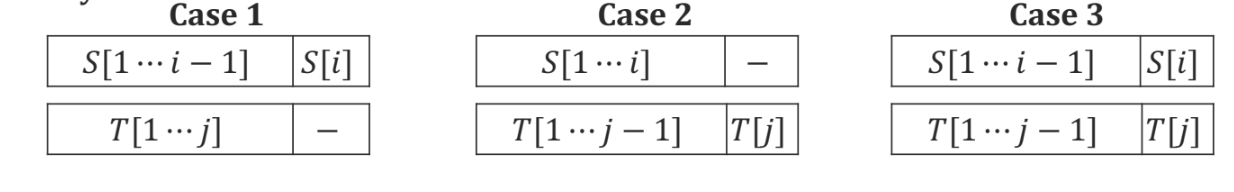
\includegraphics[scale=0.5]{alignment.png}
					\end{center}
					\comment{We add in one at a time, so there can only be one dangling letter (or none) 
					at a time!} 
			\end{itemize}
		\item We recurse based on the cases:
			\begin{itemize}
				\item Case 1: $S(i, j) = S(i-1, j) + 1$.
				\item Case 2: $S(i, j) = S(i, j-1) + 1$. 
				\item Case 3: $S(i, j) = S(i-1, j-1) + 1(S[i] \neq T[j])$.
				\item Base cases: $S(i, 0) = i$, $S(0, j) = j$. 

				The 1 represents an indicator function that counts the number of misaligned characters.
			\end{itemize}
		\item During the recursion step, we want to fill $S(i, j)$ with the \textit{minimum} value 
			of these three, since we want to minimize the number of edits. We will store this information 
			(memoizing) in a 2D array.
		\item We have to traverse our array either row by row, column by column, or diagonally. This is because
			we need to ensure that all three subproblems that we're considering have already been 
			computed. 
		\item Pseudocode:
			\begin{center}
				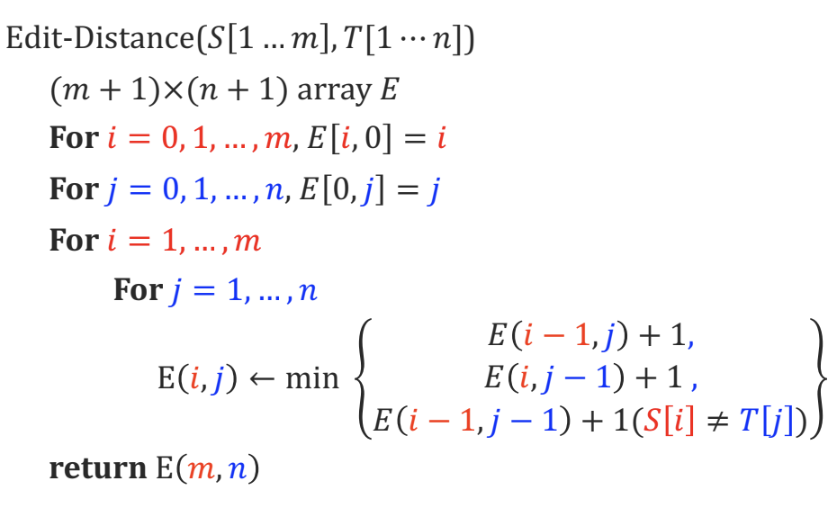
\includegraphics[scale=0.5]{alignment-pseudocode.png}
			\end{center}
		\item Runtime: there are $O(mn)$ subproblems, since we have a 2D array of dimension $mn$. At each 
			subproblem, we are only computing a minimum, which is $O(1)$ runtime, so we just have 
			$O(mn)$ runtime. 
			
			\question{Isn't the indicator also computed at this step? Why is that not accounted in the runtime?}

			\answer{The indicator is run in constant time, since we're only looking at the $i$-th character 
			in comparison to the $j$-th character.}
	\end{itemize}
	\subsection{Knapsack (with repetition)}
	\begin{itemize}
		\item A weight capacity $W$ and $n$ items with weights and values $(w_i, v_i)$. We want to output
			the most valuable collection of items whose total weight is at most $W$.
		\item We will be selecting with repetition here, but there is an easier variation where we don't
			consider repetition.
	\end{itemize}
	\subsubsection{Subproblems}
	\begin{itemize}
		\item For all $c \le W$, we want to consider the best achievable arrangement for knapsack of 
			capacity $c$. 
		\item Recurrence: For a given item $i$, then once we put it in the knapsack there are only $
			c - w_i$ capacity that remains to be optimized. This is our recurrence relation.
			\[
				K(c) = \max_{i : w_i \le c}\{v_i + K(c - w_i)\} 
			\] 
			This is a maximum over the value because we want to maximize the value being put in our 
			knapsack.
		\item We will store this information in an array of size $W + 1$, since we need a $K(0)$ element.
			\begin{center}
				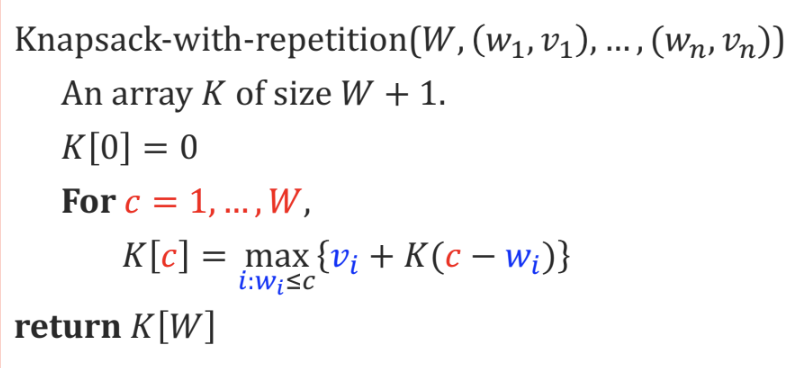
\includegraphics[scale=0.5]{knapsack-repetition.png}
			\end{center}
		\item Runtime: There are $O(W)$ subproblems, and at each subproblem, we have maximally $n$ items
			 we need to check. So in total, we have $O(nW)$ runtime.
		 \item Generally we want to think of the runtime in terms of the input. For graph problems, we looked 
			 at the input size $|V|$ and $|E|$. But for this problem, $W$ takes $\log(W)$ bits to represent 
			 $W$. So the input size is $\log(W)$. For the weights of the items themselves,
			they also only have at most $\log(W)$ bits, Therefore, the total runtime is $O(n \log W)$. 

			This kind of algorithm is polynomial in $n$, but not $W$. This is called a \underline{pseudo-
			polynomial} algorithm, since it's an algorithm that's polynomial given the numerical value 
			of the input but not in the input size.
	\end{itemize}
